% 由于表格换行符太多,使用XeLaTex报错,只能用LuaLaTeX了
% 
\subsection{工业数据案例分析}
% 
% 
% 
\begin{frame}{数据介绍}
\ \ \ \ \ \ 研究所用到数据来源于美国国家航空航天局和UC Berkeley大学实验室 \par
\ \ \ \ \ \ 松浦MC-510V 加工中心铣削加工的刀具磨损实验
% 
\begin{figure}[htbp]
% \centering
\begin{minipage}[t]{0.45\textwidth}
\centering
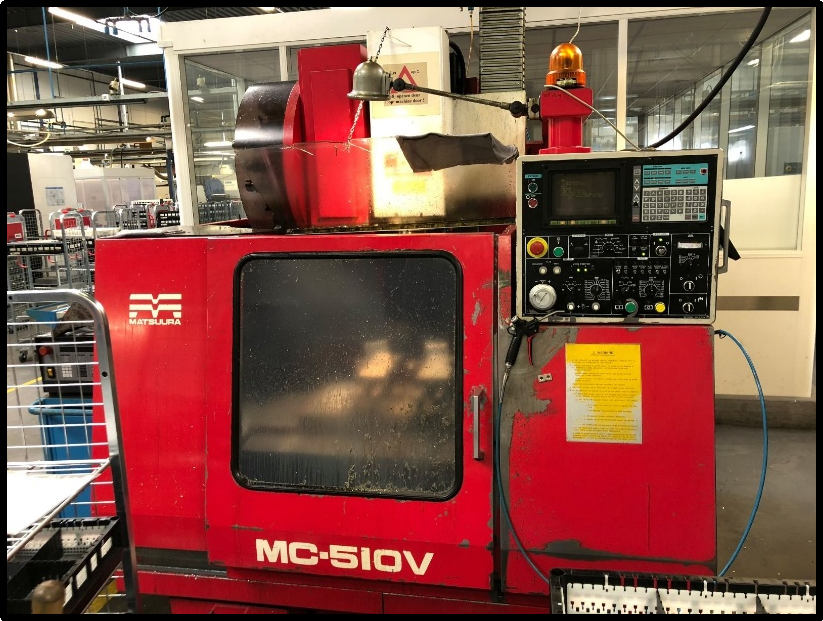
\includegraphics[height=5cm]{刀具磨损量预测神经网络/机床1.png}
% \label{fig_22}
% \caption{信号处理:smcAC}
\end{minipage}
\begin{minipage}[t]{0.45\textwidth}
\centering
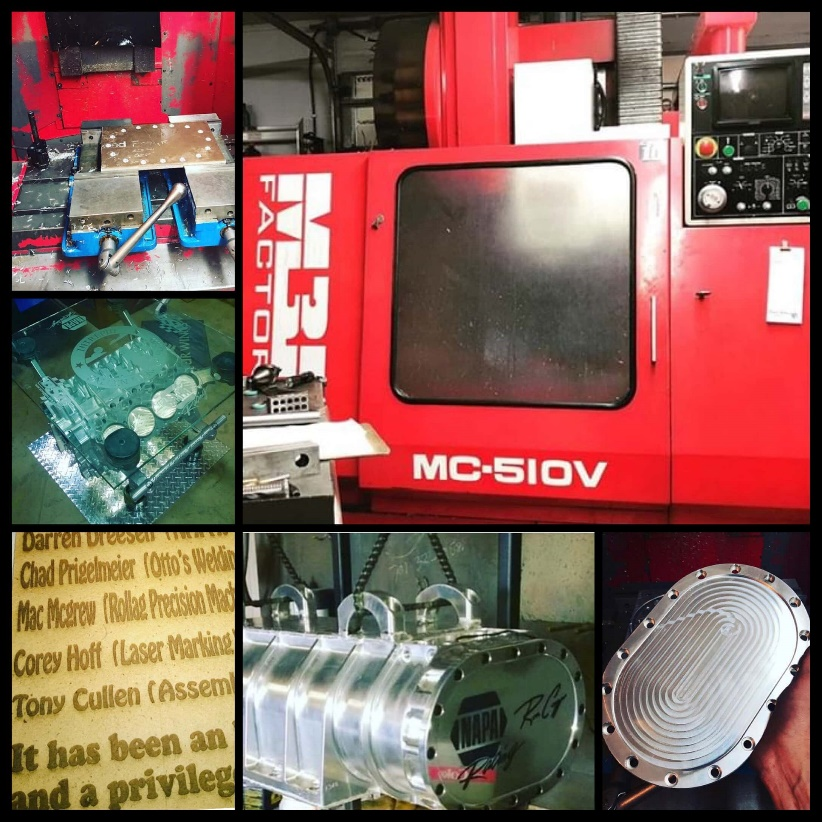
\includegraphics[height=5cm]{刀具磨损量预测神经网络/机床2.png}
%   \caption{信号处理:vib\_table}
% \label{fig_23}
\end{minipage}
\caption{松浦MC-510V 加工中心}
\end{figure}
% 
\end{frame} 
% 
% 
\begin{frame}{数据介绍}
\ \ \ \ \ \ 在操作过程中,采用传感器技术,利用声音传感器、振动传感器、电流传感器对不同操作条件下的铣床运行进行观察与记录,得到了在常规切削、进口切削以及出口切削时的刀具磨损相关数据,并将这些数据实时写入Matlab的mill.mat文件中。\par
\ \ \ \ \ \ \href{https://github.com/QianZeHao123/OpenIE/tree/main/nc_machining_center/DATA}{完整数据:https://github.com/QianZeHao123/OpenIE/DATA}\par
% 
\begin{figure}[htp]
    \centering
    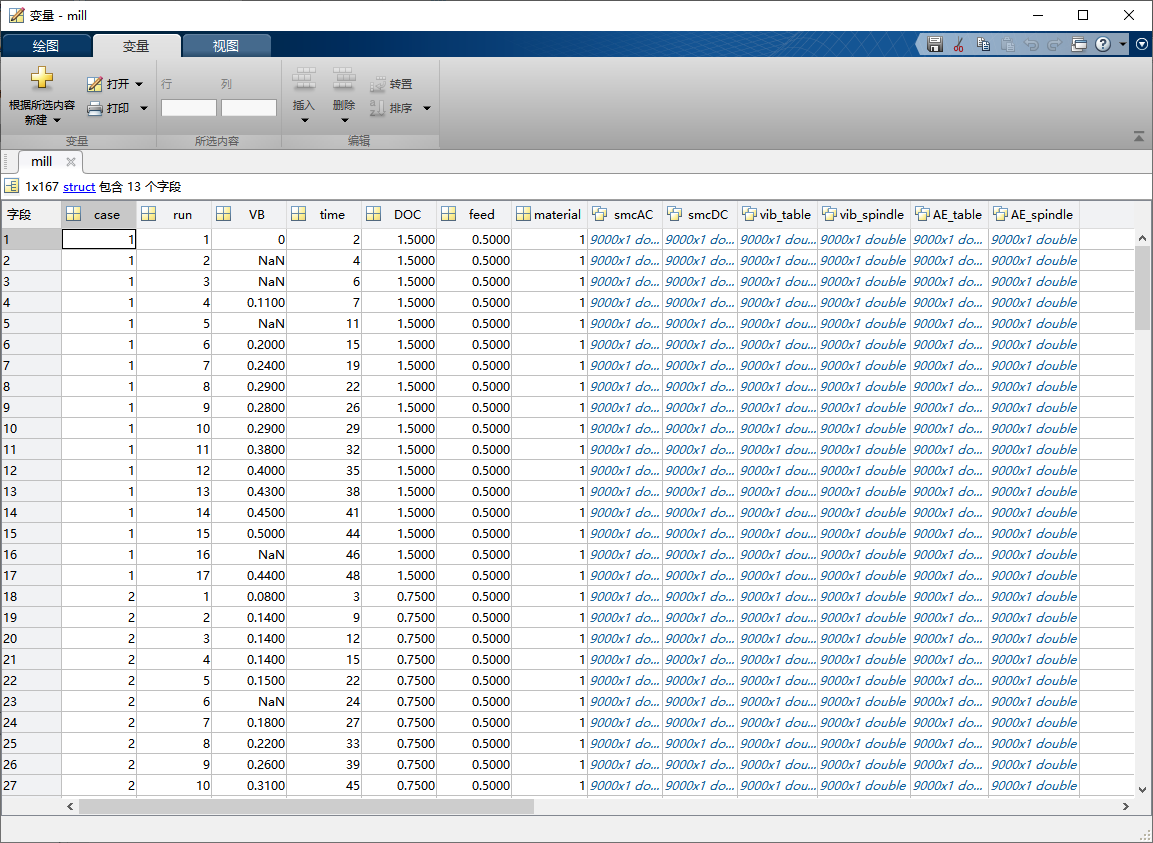
\includegraphics[width=8cm]{刀具磨损量预测神经网络/mill.png}
    \caption{Matlab mill中的数据}
\end{figure}
% 
\end{frame} 
% 
% 
% 
\begin{frame}{数据介绍}
\ \ \ \ \ \ 在实验操作过程中,铣床上刀具切削的操作条件是从工业适用性角度出发,以制造商推荐的设置为指导,具体如下:
% \begin{table}[]
%     \centering
%     % \small
%     \begin{tabular}{c|c}
%         \hline
%         属性 & 描述 \\
%         \hline
%         切割速度 & 200m/min \to 826r/min \\
%         切割深度 & 1.5mm、0.75mm \\
%         进给量 & 0.5mm/rev、0.25mm/rev \to 413mm/min、206.5mm/min \\
%         材料 & 铸铁、不锈钢J45 \\
%         刀片类型 & KC710 \\
%         铣床工作台尺寸 &  483mm*178mm*51mm \\
%         \hline
%     \end{tabular}
%     \caption{数据结构描述介绍}
% \end{table}
\begin{table}[!h]
\centering
\caption{数据结构描述介绍}
\begin{tabular}{|p{0.25\textwidth}|p{0.65\textwidth}|}
\hline 
 属性 & 描述 \\
\hline 
 切割速度 & 200m/min $\displaystyle \rightarrow $ 826r/min \\
% \hline 
 切割深度 & 1.5mm、0.75mm \\
% \hline 
 进给量 & 0.5mm/rev、0.25mm/rev $\displaystyle \rightarrow $ 413mm/min、206.5mm/min \\
% \hline 
 材料 & 铸铁、不锈钢J45 \\
% \hline 
 刀片类型 & KC710 \\
% \hline 
 铣床工作台尺寸 & 483mm*178mm*51mm \\
 \hline
\end{tabular}
\end{table}
% 
\ \ \ \ \ \ 为了便于建立模型,我们对相关变量进行了说明,具体如下:
% 
case(案例数量)、run(每个案例中的运行次数)、VB(刀具磨损)、time(测量时刻)、DOC(切削深度)、feed(进给量)、material(材料)、smcAC(主轴交流电信号)、smcDC(主轴直流电信号)、vib\_table(工作台振动信号)、vib\_spindle(主轴振动信号)、AE\_table(工作台噪音信号)、AE\_spindle(主轴噪音信号)、case(案例数量)
\end{frame}
% 
% 
% \begin{frame}{数据介绍}
% \ \ \ \ \ \ 为了便于建立模型,我们对相关变量进行了说明,具体如下表所示
% % 
% \begin{table}[]
%     \centering
%     \begin{tabular}{cc|cc}
%         \hline
%         符号 & 含义 & 符号 & 含义 \\
%         \hline
%         case & 案例数量 & smcAC & 主轴交流电信号 \\
%         run	& 每个案例中的运行次数 & smcDC & 主轴直流电信号 \\
%         VB & 刀具磨损 & vib\_table & 工作台振动信号 \\
%         time & 测量时刻 & vib\_spindle & 主轴振动信号 \\
%         DOC & 切削深度 & AE\_table & 工作台噪音信号 \\
%         feed & 进给量 & AE\_spindle & 主轴噪音信号 \\
%         material & 材料 \\
%         \hline
%     \end{tabular}
%     \caption{数据结构说明}
% \end{table}
% % 
% \end{frame}
% 
% 
% 
\begin{frame}{数据处理}
\ \ \ \ \ \ 训练刀具磨损量测定神经网络模型使用的是个人PC,配置如下:CPU(Intel(R) Core(TM) i5-9400F CPU @ 2.90GHz),GPU(NVIDIA GeForce GTX 1660),内存8.0 GB。 \par
\ \ \ \ \ \ 我们团队使用Matlab编写绘制了所有输出信号的脚本,用于人工筛选可以用来被训练的数据。\par
% 
\begin{figure}[htp]
    \centering
    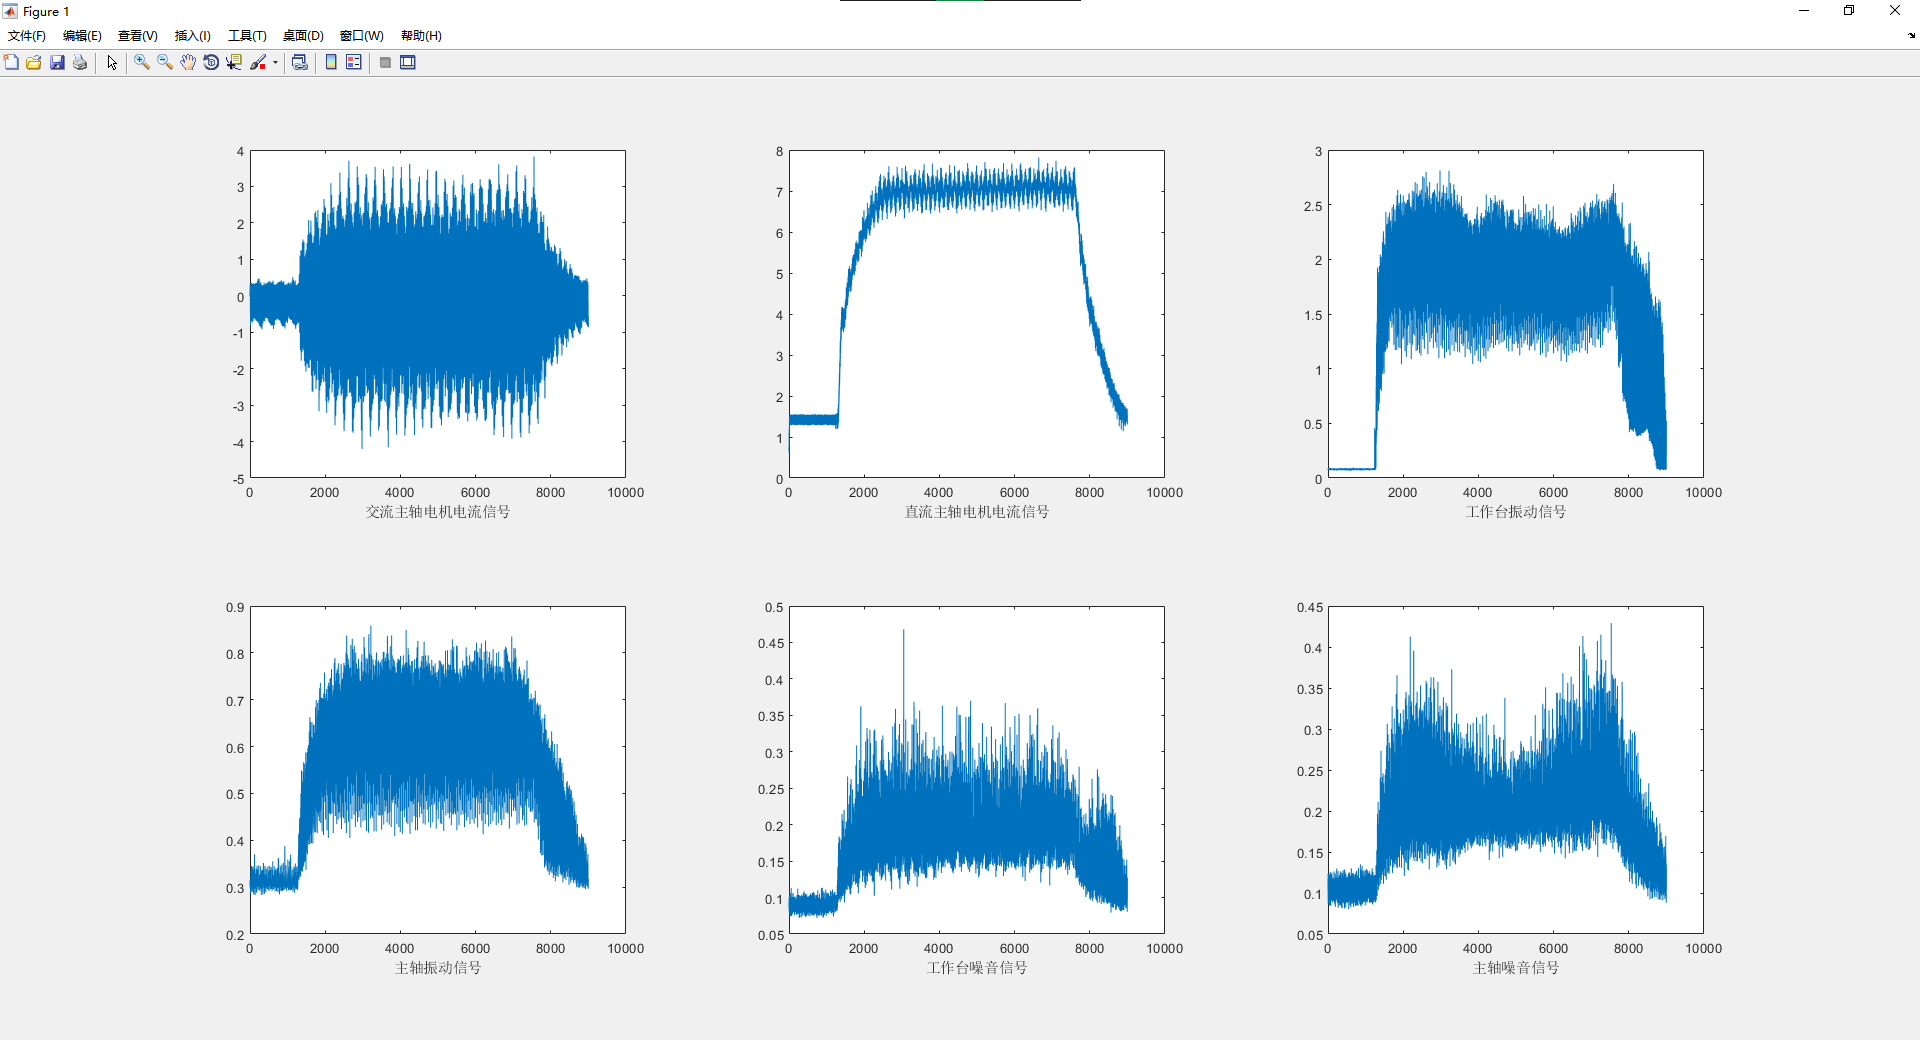
\includegraphics[width=10cm]{刀具磨损量预测神经网络/signal.png}
    \caption{机床传感器信号图像}
\end{figure}
% 
\end{frame}
% 
% 
% 
% 
% \subsection{特征工程}
% \subsubsection{信号处理}
% 
% 
% \begin{frame}{信号处理——时域特征提取}
% \ \ \ \ \ \ 对于时域特征的提取,我们将有量纲特征值与无量纲特征值相结合,以时间为自变量表示目标信号数据的波形,具体特征如下:
% \begin{minipage}[t]{0.45\textwidth}
% \centering
% $$ 绝对均值: |\bar{x}|=\frac{1}{N} \sum_{i=1}^{N}\left|x_{i}\right| $$\par
% $$ 峭度值:x_{ra}=\left(\frac{1}{N} \sum_{i=1}^{N} \sqrt{|x_i|}\right)^{2} $$\par
% $$ 均方根值:x_{rms}=\sqrt{\frac{1}{N} \sum_{k=1}^{N} x_{i}^{2}} $$\par
% $$ 方根幅值:x_{kurtosis}=\frac{1}{N} \sum_{k=1}^{N}(x)^{n} $$\par
% \end{minipage}
% \begin{minipage}[t]{0.45\textwidth}
% \centering
% $$ 峰值:x_{pesk}=X_{max} $$\par
% $$ 波形因子:f_{shape}=\frac{x_{rms}}{|\bar{x}|} $$\par
% $$ 脉冲因子:f_{pulse}=\frac{x_{peak}}{|x|} $$\par
% $$ 峰值因子:f_{crest}=\frac{x_{peak}}{x_{rms}} $$\par
% $$ 裕度因子:f_{celearance}=\frac{x_{peak}}{x_{ra}} $$\par
% \end{minipage}
% \end{frame} 
% % 
% % 
% \begin{frame}{信号处理——频域特征提取}
% \ \ \ \ \ \ 但是只有时域特征的铣削力存在波动较大以及不同刀具差异较大的情况,因此,只有时域特征不够完善,需进一步建立频域和时频域的特征提取。\par
% \ \ \ \ \ \ 我们采取频谱分析法提取铣刀切削原始信号的频域特征,具体特征如下:
% \begin{minipage}[t]{0.45\textwidth}
% \centering
% $$ 重心频率:F_{FC}=\frac{\int_{0}^{+\infty}f(t)FFT(t)dt}{\int_{0}^{+\infty} FFT(t)dt} $$\par

% \end{minipage}
% \begin{minipage}[t]{0.45\textwidth}
% \centering
% $$ 均方频率:F_{MSF}=\frac{\int_{0}^{+\infty} FFT(t)f(t)^{2}dt}{\int_{0}^{+\infty}FFT(t)dt} $$\par
% \end{minipage}
% $$ 均方根频率:F_{RMSF}=\sqrt{\frac{\int_{0}^{+\infty}FFT(t)f(t)^{2}dt}{\int_{0}^{+\infty}FFT(t)dt}} $$ \par
% $$ 频率方差: F_{VF}=\frac{\int_{0}^{+\infty}(f(t)-\frac{\int_{0}^{+\infty}f(t)FFT(t)dt}{\int_{0}^{+\infty}FFT(t)dt} )^{2}dt}{\int_{0}^{+\infty}FFT(t)dt}  $$ \par
% \end{frame}
% % 
% % 
% \begin{frame}{Matlab信号处理}
% \begin{figure}[htbp]
% % \centering
% \begin{minipage}[t]{0.48\textwidth}
% \centering
% 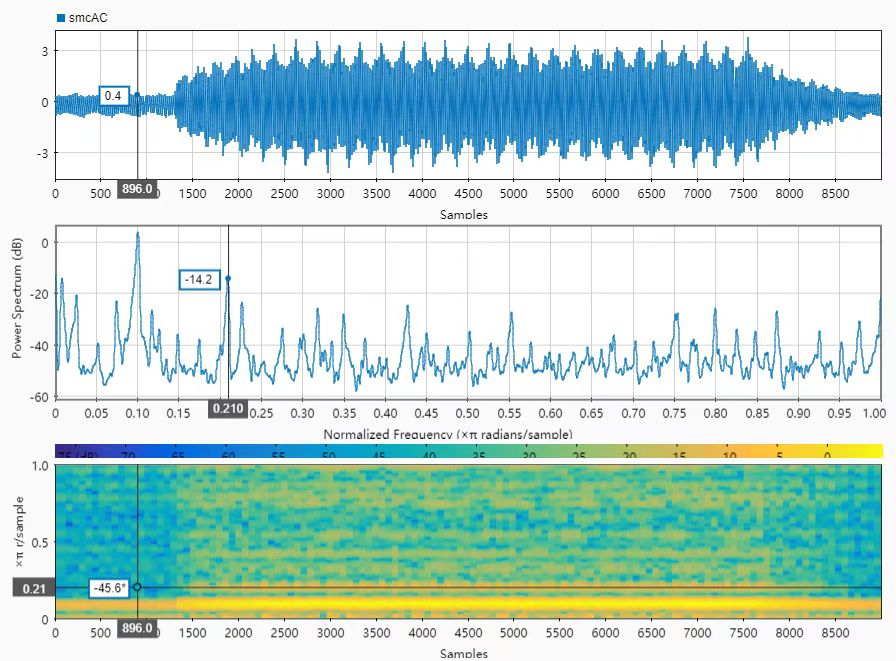
\includegraphics[width=6cm]{刀具磨损量预测神经网络/smcAC.jpg}
% % \label{fig_22}
% \caption{信号处理:smcAC}
% \end{minipage}
% \begin{minipage}[t]{0.48\textwidth}
% \centering
% 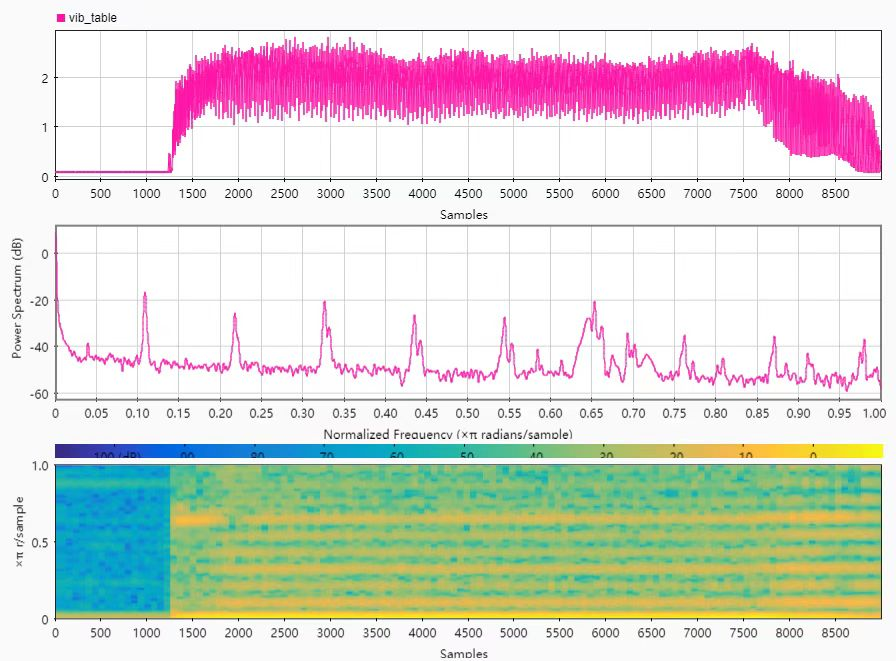
\includegraphics[width=6cm]{刀具磨损量预测神经网络/vib_table.jpg}
%   \caption{信号处理:vib\_table}
% % \label{fig_23}
% \end{minipage}
% \end{figure}
% \end{frame}
% % 
% % 
% % \subsubsection{特征筛选}
% \begin{frame}{特征筛选}
% \ \ \ \ \ \ 每一次的铣削过程都对应着数万条信号数据和一个真实的铣刀磨损值,但并非所有采集到的信号数据都与刀具磨损量有着相关的关系,且经过各式传感器采集得到的原始信号的数据量过于庞大,原始信号数据当中还夹杂存在着各种干扰噪声,将其直接应用于刀具磨损量分析预测会大大增大方法实现的难度。因而需要通过进行合理适当的特征工程,在海量原始信号数据当中筛选出对研究目标对象刀具磨损量较为敏感的特征。
% F-test检验方法的原理是:假设特征矩阵为X,目标值为y,特征序号为i,使用函数mean()、std()和size()来分别表示计算特征矩阵平均值、特征矩阵标准差和目标长度,均值中心化则使用centered来表示。\par
% \ \ \ \ \ \ 因此相关系数Corr的公式为:\par
% $$ Corr=\frac{(X[:, i]-mean(X[:, i]))^{*}(y-mean(y))}{std(X[:, i])^{*} std(y)} $$ \par
% % 
% \ \ \ \ \ \ 自由度n的公式为:\par
% $$ n=size(y)-\left\{\begin{array}{l}
% 2\ \ \ if\ X,\ y\ centered \\
% 1\ \ \ if\ X,\ y\ not\ centered 
% \end{array}\right. $$ \par
% % 
% \ \ \ \ \ \ 基于此可以评估检验特征矩阵与目标值之间具有的线性关系,F-test评估检验值大于0.5的标准来进行特征选择。通过建立上述特征选择分析论证得出在各通道信号中声发射信号并没有贡献出与刀具磨损量相关的最优特征,因此在本研究的实验阶段将舍弃声发射信号通道的数据。\par
% % 
% \end{frame}
% \subsection{BPNN反向传播神经网络模型}
\begin{frame}{循环神经网络模型训练}
\ \ \ \ \ \ 经过数据筛选和特征工程,共获得145组数据,每组数据有60个参数,我们使用Matlab编写脚本,将这些数据转化为145rows~*~60colums的矩阵作为训练神经网络的输入,输出为与145组数据的相对应的刀具磨损量VB的值。\par

\begin{figure}[htbp]

\begin{minipage}[t]{0.48\textwidth}
\centering
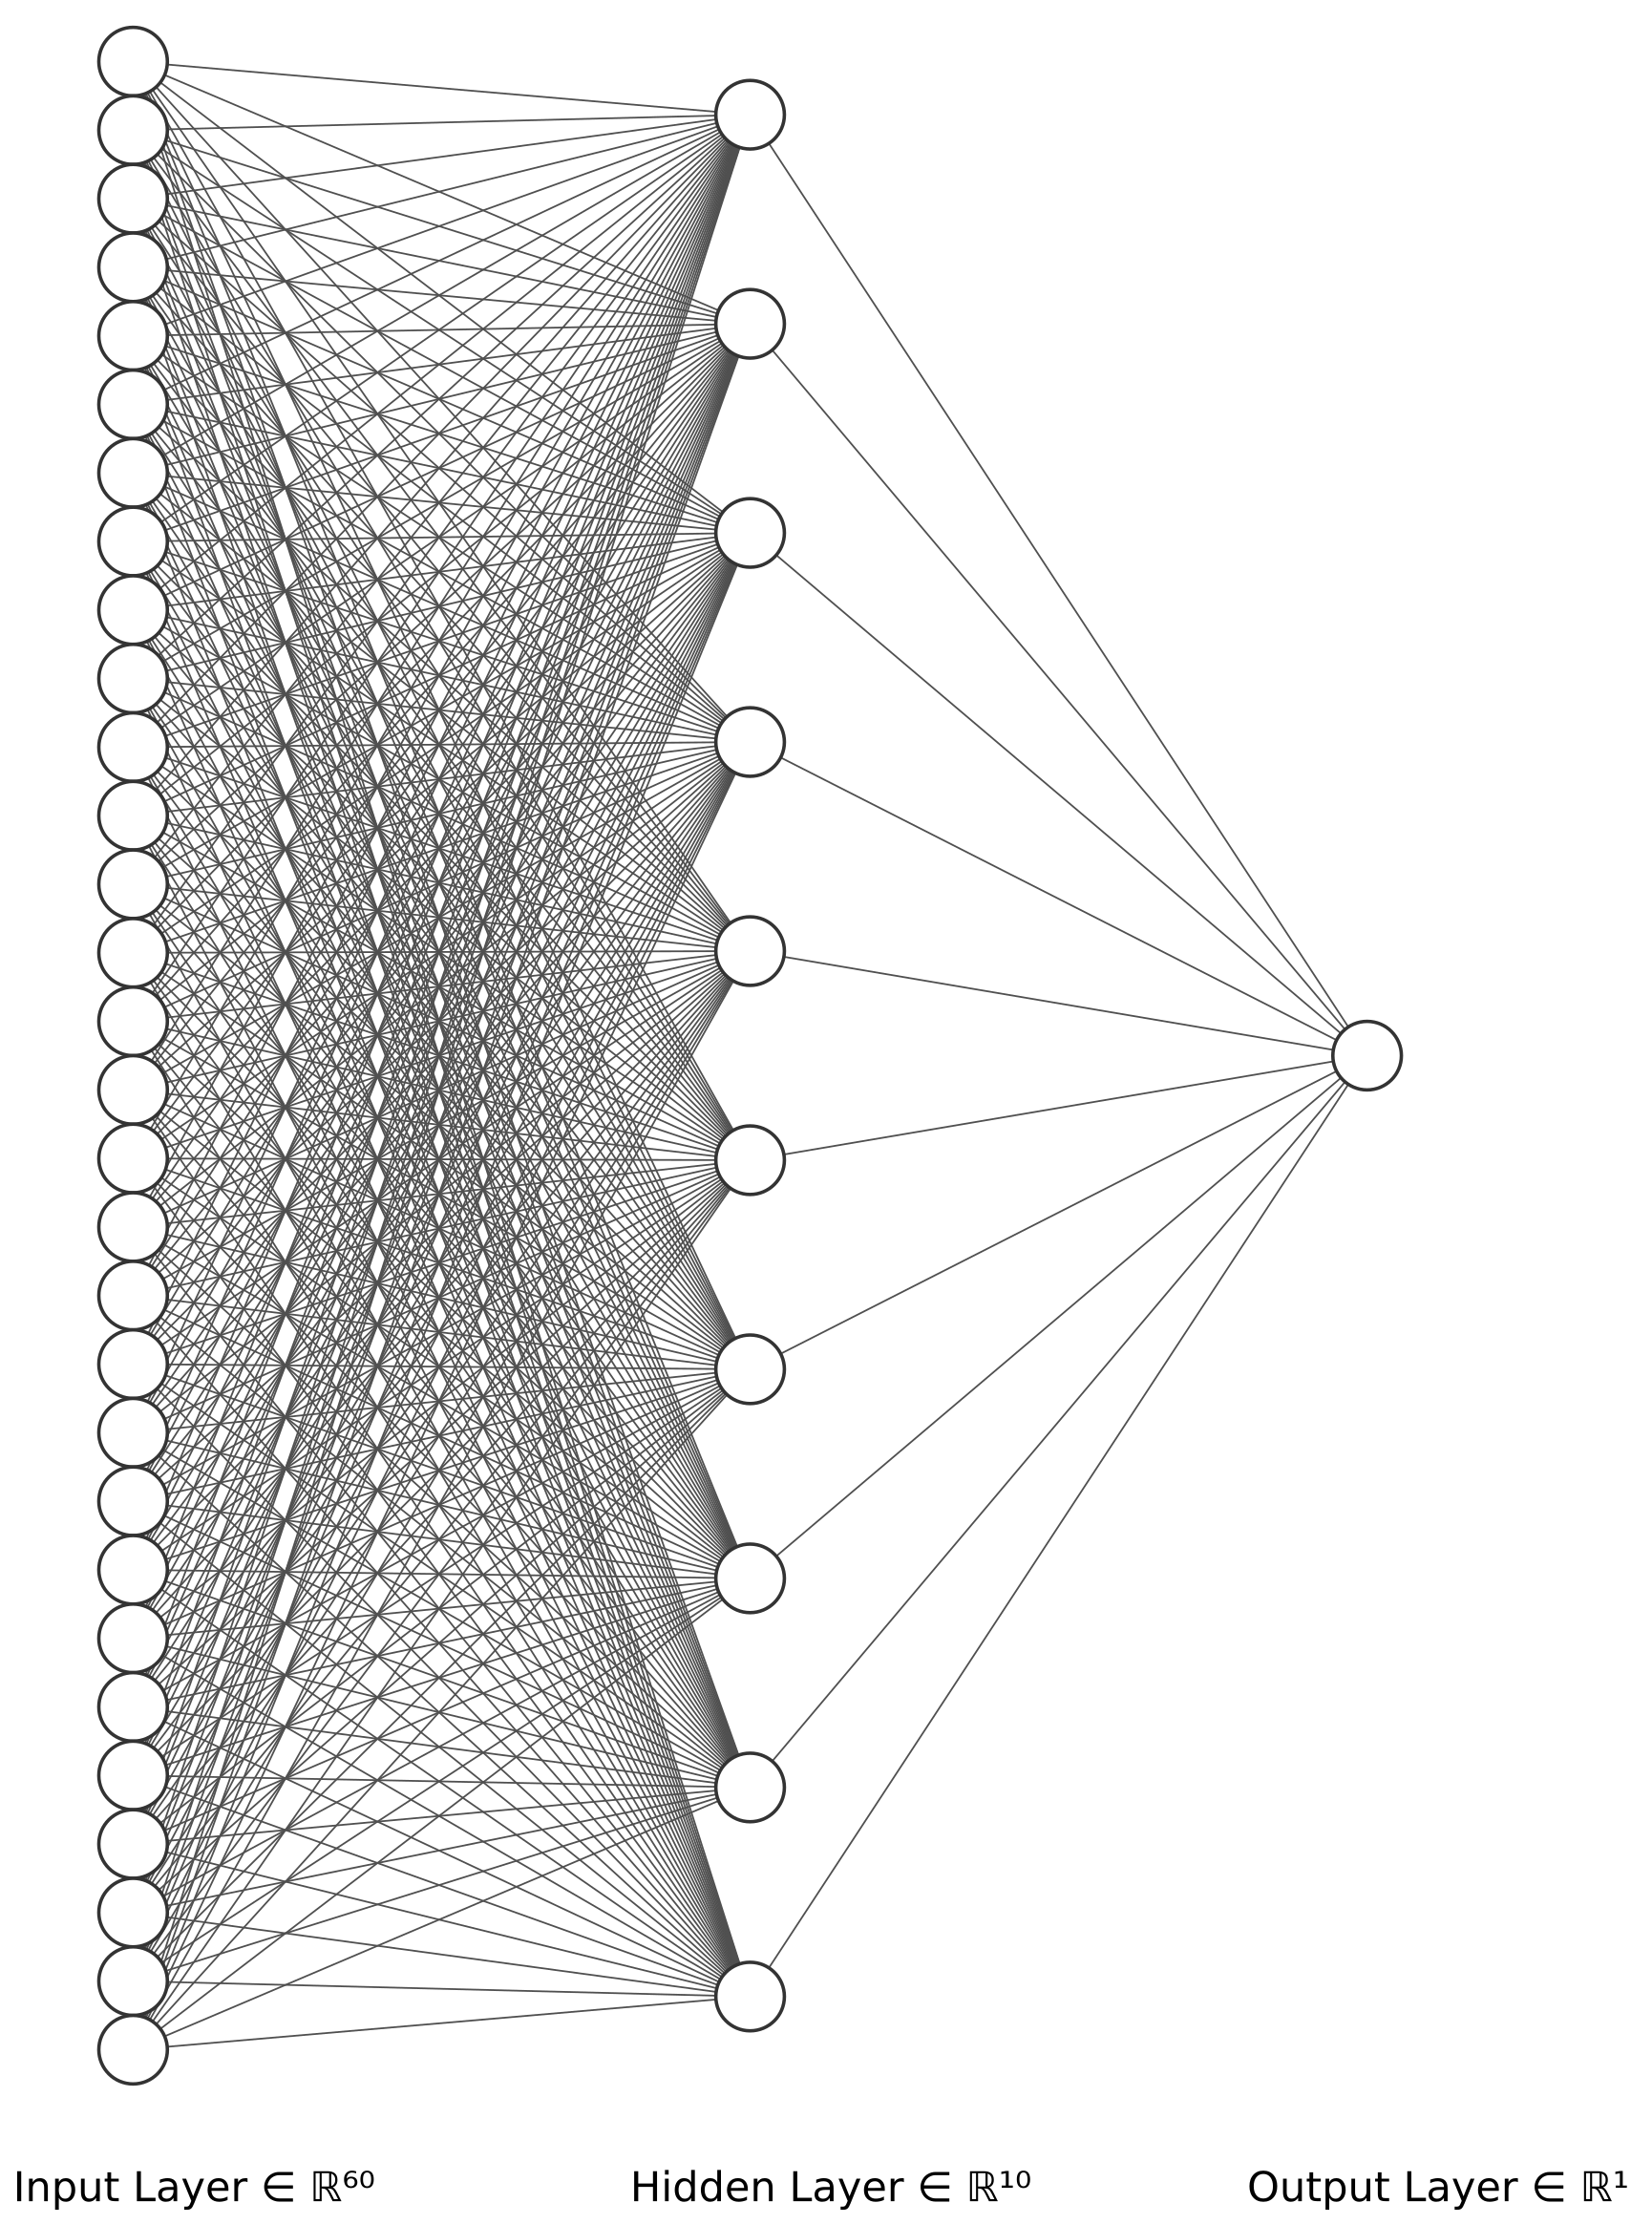
\includegraphics[height=6cm]{刀具磨损量预测神经网络/nn.png}

\caption{神经网络结构图}
\end{minipage}
\begin{minipage}[t]{0.48\textwidth}
\centering
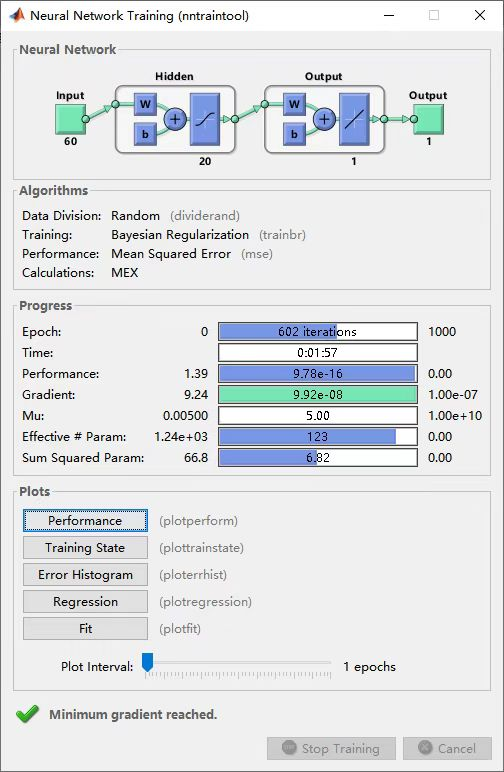
\includegraphics[height=6cm]{刀具磨损量预测神经网络/res.jpg}
\caption{神经网络训练结果}

\end{minipage}
\end{figure}

% 
\end{frame}
